\chapter{Introduction}
LHCb is one of the four major experiments at Conseil Européen pour la Recherche Nucléaire (CERN) specialized in precision measurements and usually studies b- and c- quark hadrons. During run 2 (2015-2018), a large set of data has been collected after the initial selection process using the trigger system. However, the data has large amount of background, resulting in a shape of the invariant mass distribution where the peak of the $B_{s}^{0} \rightarrow \psi(2S)K_{s}^{0}$ decay is hidden.\\

The tree level Feynman diagram of the decay is shown in Figure \ref{decay}. This decay can be used to study all important CP violation. One example is the measurement of the time-dependent CP asymmetry in the decay.\\

\begin{figure}[H]
    \centering
    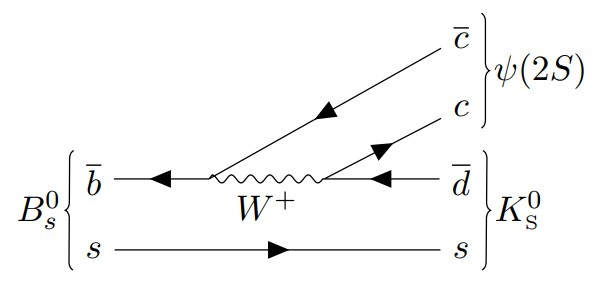
\includegraphics[width=0.5\linewidth]{Figure/decay.jpg}
    \caption{Leading order Feynman diagram of the decay $B_{s}^{0} \rightarrow \psi(2S)K_{s}^{0}$ in the Standard Model.}
    \label{decay}
\end{figure}

Three datasets are used for this analysis:\\
\begin{enumerate}
    \item The real data recorded by the LHCb experiment with a very rough
    selection.
    \item A sample of the signal decay $B_{s}^{0} \rightarrow \psi(2S)K_{s}^{0}$ obtained from Monte-Carlo simulation.
    \item A sample of the (kinematically) very similar decay $B^{0} \rightarrow \psi(2S)K_{s}^{0}$ obtained from Monte-Carlo simulation.
\end{enumerate}

The LHCb experiment uses an elaborate trigger system to select likely interesting events and
reduce the great amount of data to a size that is small enough to be stored. Often, the interesting events are are hidden in the real data sample
such that some further selection is required. In order to study the physics of $B_{s}^{0} \rightarrow \psi(2S)K_{s}^{0}$
events, a cleaner sample with
better signal to background ratio is required. Obtaining such a sample, using a multi-variate analysis (MVA)
to classify signal and background, is the aim of this study. A MVA classifier is a machine learning method used to distinguish between different categories or classes (e.g. signal vs. background) by analyzing multiple input variables simultaneously. The signal region should never be used in training the classifier to avoid bias. Otherwise, it might lead to false discovery.\\

Simulated data often differ from real data due to limitations in theoretical models and detector simulations. Improving accuracy would require significantly more computational resources, as simulating each event already takes several minutes and millions of events are needed per decay mode. To lower these discrepancies, kinematic weights are applied to simulation samples. These weights correct for differences between data and simulation in kinematic distributions, ensuring better alignment with real observations.\\

Since, the signal in the real dataset is hidden in the background, it is essential to use a loss function that needs to be minimized. The inverse of the loss function is called a figure of merit (FOM), which helps quantify the quality of a classifier. One important and common FOM in the high-energy physics (HEP) community is Punzi FOM \cite{punzi}. It is defined as:\\
\begin{align}
    FOM=\frac{\epsilon_{sig}}{\frac{5}{2}-\sqrt{N_{bkg}}}
\end{align}
where $N_{bkg}$ is the expected number of background events in the signal region and $\epsilon_{sig}$ is the classification efficiency of the signal. Again, $N_{bkg}$ can be defined as:\\
$$
    N_{bkg} = \text{No. of background events in the background region}\times\frac{\text{width of signal region}}{\text{width of background region}}.
$$

The background in the real dataset is mostly combinatorial. Combinatorial background consists of events that pass the selection purely due to coincidence. For example, two unrelated muons may accidentally appear to originate from a common vertex, prompting the reconstruction algorithm to falsely identify them as a $\psi(2S)$ candidate. If a nearby, randomly associated $K_{s}^{0}$ is also reconstructed, the algorithm may combine it with the $\psi(2S)$ to form a $B$ candidate. However, since the $\psi(2S)$ and 
$K_{s}^{0}$
  are uncorrelated in such cases, the resulting invariant mass of the reconstructed $B$ candidate can span a wide range. In contrast, true $B_{s}^{0} \rightarrow \psi(2S)K_{s}^{0}$
  decays will cluster around the nominal 
$B_{s}^{0}$
  mass, with well-defined kinematic and geometric properties. Because combinatorial background lacks such correlations, kinematic variables are particularly effective in distinguishing it from genuine signal events.\\
  
 In this experiment, there are a lot of instances where distributions will be compared. A trivial way to do that is to get the largest distance between the cumulative probability distributions(CDF). It can be defined as:\\
$$\sup_{n}\abs{{F_{n}^{1} - F_{n}^{2}}}$$
where n is the number of bins in the histogram. This can be easily obtained using the Kolmogorov-Smirnov (KS) test from the scipy package in coding \cite{ks}.\\

The final evaluation can be done using the significance which can be defined as:\\
\begin{align}
    m = \frac{N_{sig}}{\sqrt{N_{sig} + N_{bkg}}}
    \label{proxy}
\end{align}

where $N_{bkg}$ is the number of background candidates and $N_{sig}$ is the number of signal candidates. This significance is a measure of how likely the result is produced by statistical calculations. A discovery is claimed if the significance is greater than 5. If the significance is larger than 3, then there is evidence of the signal.\\